\documentclass[12pt]{article}

\usepackage[utf8]{inputenc}
\usepackage[T1]{fontenc}
\usepackage[francais]{babel}

\renewcommand{\emph}{\textbf}

\title{\textbf{Thème 3 : Féminin et masculin}}
\date{}
\usepackage{graphicx}
\begin{document}

\maketitle

\section*{IV. Maîtriser la procréation}

\subsection*{a) La contraception}

\textit{Cf. doc. 14 et 15.}

\subsection*{b) La PMA}

\textit{Cf. activité.}

\paragraph{Bilan.}
La connaissance scientifique des mécanismes de contrôle de l'activité des gonades a permis la mise au moint de méthodes contraceptiveset d'aider les couples infertiles à procréer.

\subsubsection*{Exercice}

\begin{enumerate}
\item Homme \emph{stérile} (?), femme fertile\\
$\rightarrow$ Don de sperme + insémination artificielle
\item Homme fertile, femme a des \emph{problèmes hormanaux}\\
$\rightarrow$ Stimulation ovarienne.
\item Homme \emph{peu fertile}, femme ayant une {double obturation des trompes} (pb anatomique)\\
$\rightarrow$ Stimulation ovarienne + FIVETTE + ICSI
\end{enumerate}

\paragraph{Observation du document 2.}
Le produit passe dans les trompes chez une femme fertile, mais pas chez la femme du couple \#3. Les trompes de cette femme sont donc bouchées.

\section*{V. Bases biologique du plaisir sexuel}

\textit{Cf. activité.}

\begin{quotation}
Thomas : les gays prennent-ils du plaisir ?\\
Réponse : Et oui, les fesses sont des zones hérogènes.
\end{quotation}

\begin{figure}[htp]
\centering
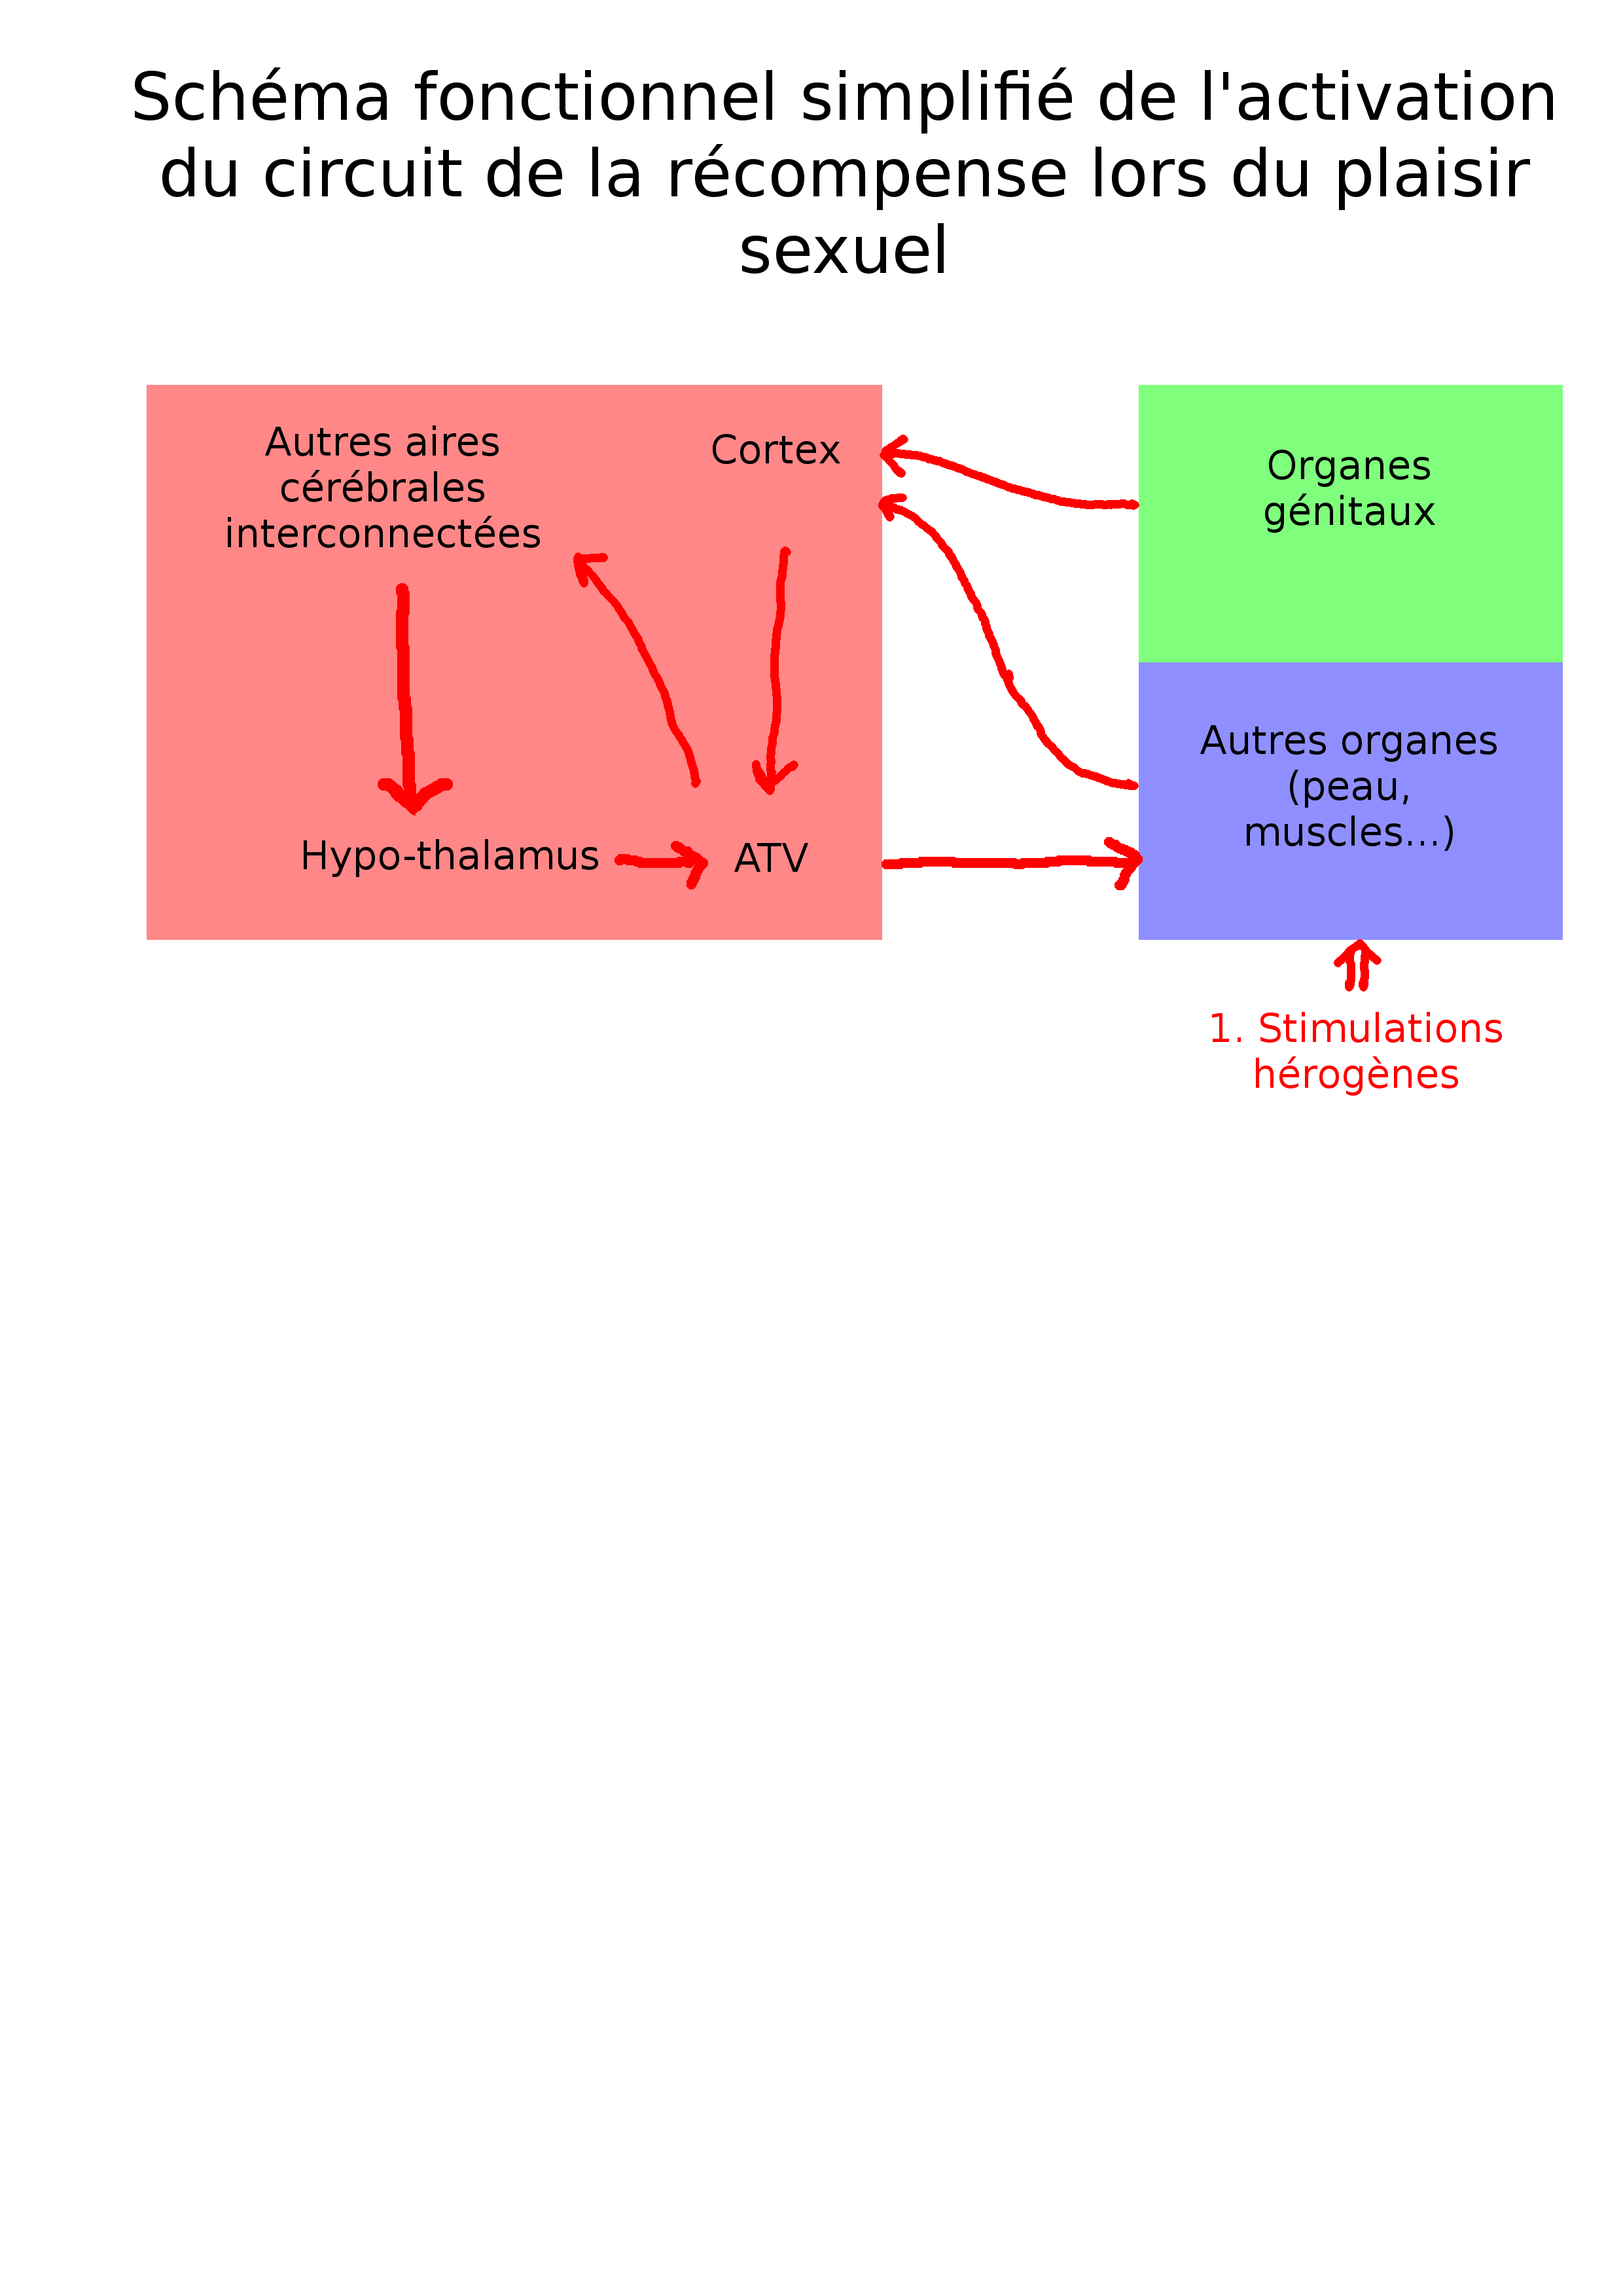
\includegraphics[scale=0.7]{img/circuit-de-la-recompense.png}
\caption{Le circuit de la recompense}
\label{}
\end{figure}

\end{document}